\chapter{Fundamentação Teórica}\label{cap:fundamentacao}

Este capítulo apresenta os conceitos usados na construção e na análise do conjunto de dados. A discussão cobre navegação visual, visão monocular, fluxo óptico, representação tridimensional, aprendizado com dados tabulares e explicabilidade.

\section{Navegação visual em drones}

A navegação autônoma integra percepção, decisão e controle. Em ambientes densos, imagens de drones podem apresentar oclusões, objetos finos, mudanças de iluminação, vibração e borramento. Em voos rápidos, a informação também precisa chegar a tempo de permitir uma reação \cite{Loquercio2021,Ramachandran2021}.

Abordagens tradicionais dividem o problema em percepção, mapeamento, planejamento e controle. Essa organização facilita o desenvolvimento, mas pode introduzir latência e acumular erros. Estratégias reativas aproximam a percepção da ação e são úteis para produzir respostas rápidas, embora não substituam todas as funções de um sistema de navegação.

\section{Visão monocular e profundidade}

Uma câmera monocular registra a cena em duas dimensões e não preserva diretamente a escala métrica. A profundidade precisa ser inferida por perspectiva, textura, tamanho relativo, sombreamento, movimento ou conhecimento aprendido \cite{Vyas2022,Arampatzakis2024}. Estimadores recentes de profundidade monocular alcançam bons resultados, mas ainda enfrentam problemas de generalização, incerteza e custo computacional \cite{RealTimeMonocular2022,Liu2023,Dhanushkodi2025}. O Depth Anything V2 combina um modelo professor de maior capacidade, imagens sintéticas e pseudo-rótulos em imagens reais. Seus autores também disponibilizam variantes ajustadas para profundidade métrica \cite{DepthAnythingV2}. 

\section{Representação tridimensional e planejamento}

Um mapa de profundidade associa uma distância a cada pixel, mas essas distâncias ainda estão no referencial da câmera. Com os parâmetros intrínsecos, cada pixel pode ser reprojetado como um ponto tridimensional. A pose da câmera permite transformar esses pontos para um referencial comum e acumular observações ao longo do voo. Uma grade de ocupação divide o espaço em células livres, ocupadas ou ainda não observadas e atualiza essas hipóteses conforme novas observações chegam \cite{Elfes1989}. Estruturas baseadas em octrees permitem representar esse tipo de mapa com diferentes níveis de resolução \cite{Hornung2013}.

O planejamento procura conectar origem e destino respeitando as regiões livres da representação. Entre as estratégias de busca em grafos está o A*, que combina custo acumulado e estimativa do custo restante \cite{Hart1968}. Estratégias de exploração podem escolher objetivos próximos à fronteira com o desconhecido \cite{Yamauchi1997}. A travessia de voxels permite verificar as células percorridas por um segmento \cite{AmanatidesWoo1987}. A configuração adotada neste estudo é apresentada no capítulo de implementação.

\section{Fluxo óptico e movimento visual}

O fluxo óptico descreve o deslocamento aparente de pontos ou regiões entre quadros. Lucas--Kanade estima deslocamentos locais \cite{LucasKanade1981}, enquanto Shi--Tomasi seleciona pontos adequados ao rastreamento \cite{ShiTomasi1994}. Obstáculos próximos tendem a produzir movimento aparente maior durante o avanço, mas o fluxo também depende da rotação, da translação e da geometria da cena.

Resolução, frequência, borramento e incerteza das correspondências afetam a qualidade do sinal \cite{SimoneGodio2022,Peidong2021,Estimation2109}. Por isso, o fluxo deve ser analisado junto à atitude e ao movimento do veículo. A odometria visual estima o movimento da câmera a partir de imagens sucessivas. Essa combinação também aparece em odometria visual e em sistemas de prevenção de colisões \cite{Tarrio2015,Garcia2016,Xiao2021}.

\section{Aprendizado com dados tabulares}

Uma MLP permite verificar se atributos resumidos contêm informação suficiente para estimar os alvos sem processar a imagem completa. A rede aprende relações não lineares entre os atributos, mas pode apresentar sobreajuste em conjuntos pequenos. O \textit{dropout} e a parada antecipada ajudam a limitar esse problema \cite{Srivastava2014,Prechelt1998}.

Modelos de árvores são referências importantes porque costumam ter bom desempenho em bases tabulares de tamanho moderado \cite{OyallonandGaelVaroquaux5220}. Uma comparação justa também precisa incluir um modelo simples, como a previsão constante da média do treino. Se um modelo complexo não supera essa referência, o resultado indica que a distribuição do alvo ainda favorece previsões próximas de zero.

\section{Explicabilidade e ablação}

Gradientes em relação às entradas mostram como o erro muda perto de uma amostra. \emph{Integrated Gradients} é uma referência para métodos de atribuição baseados em gradiente \cite{Sundararajan2017}, e trabalhos posteriores discutem suas propriedades e limitações \cite{Walker5289,Axiomatic2025}. Como as entradas deste estudo são tabulares, a análise atribui importância aos atributos, e não a regiões da imagem como no Grad-CAM \cite{Selvaraju2017}.

A ablação responde a outra pergunta: o que acontece quando um grupo de entradas é removido e o modelo é treinado novamente? O gradiente mede sensibilidade local. A ablação mede a mudança no desempenho.

\section{Simulação e reprodutibilidade}

O Gazebo permite configurar física, cenário e sensores \cite{Koenig7803}, enquanto o PX4 fornece o piloto automático e a interface com aplicações externas \cite{Meier8092}. No modo \textit{Software in the Loop} (SITL), o sistema pode repetir a missão e registrar uma referência de profundidade sem colocar um veículo físico em risco.

Mesmo assim, processos concorrentes e pequenas diferenças temporais podem produzir trajetórias distintas. Por isso, cada voo completo é tratado como uma unidade experimental, e a divisão dos dados ocorre por execução.

\begin{figure}[htbp]
\centering
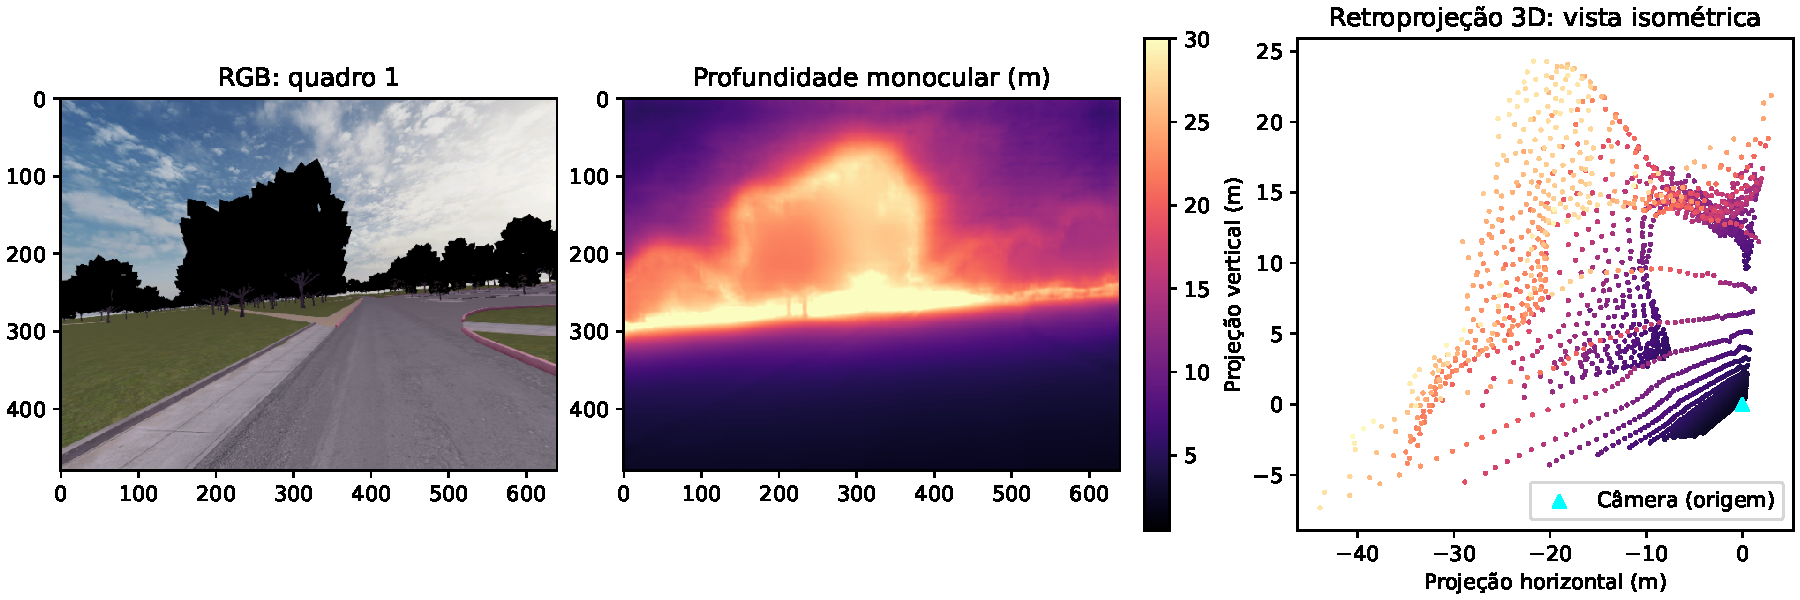
\includegraphics[width=0.98\linewidth]{figuras/metodologia_rgb_profundidade_3d.pdf}
\caption{Mesmo quadro real do replay: RGB, profundidade monocular e retroprojeção isométrica, com câmera na origem óptica e profundidade em metros.}
\end{figure}

\begin{figure}[htbp]
\centering
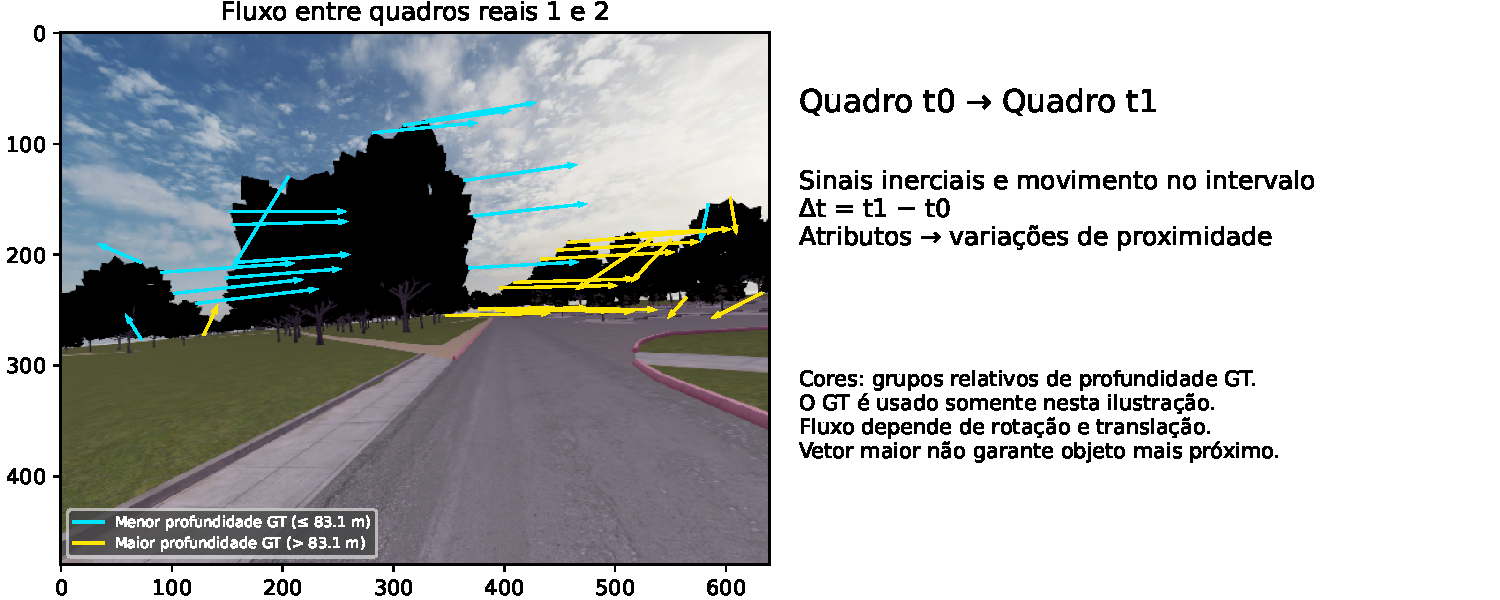
\includegraphics[width=0.98\linewidth]{figuras/metodologia_fluxo_intervalo.pdf}
\caption{Fluxo entre dois quadros reais e esquema do intervalo visual. As cores distinguem profundidades de referência abaixo e acima da mediana dos pontos válidos. O GT é usado somente para ilustrar a distância relativa. Rotação e translação influenciam os vetores, portanto um vetor maior não garante menor distância.}
\end{figure}

\begin{figure}[htbp]
\centering
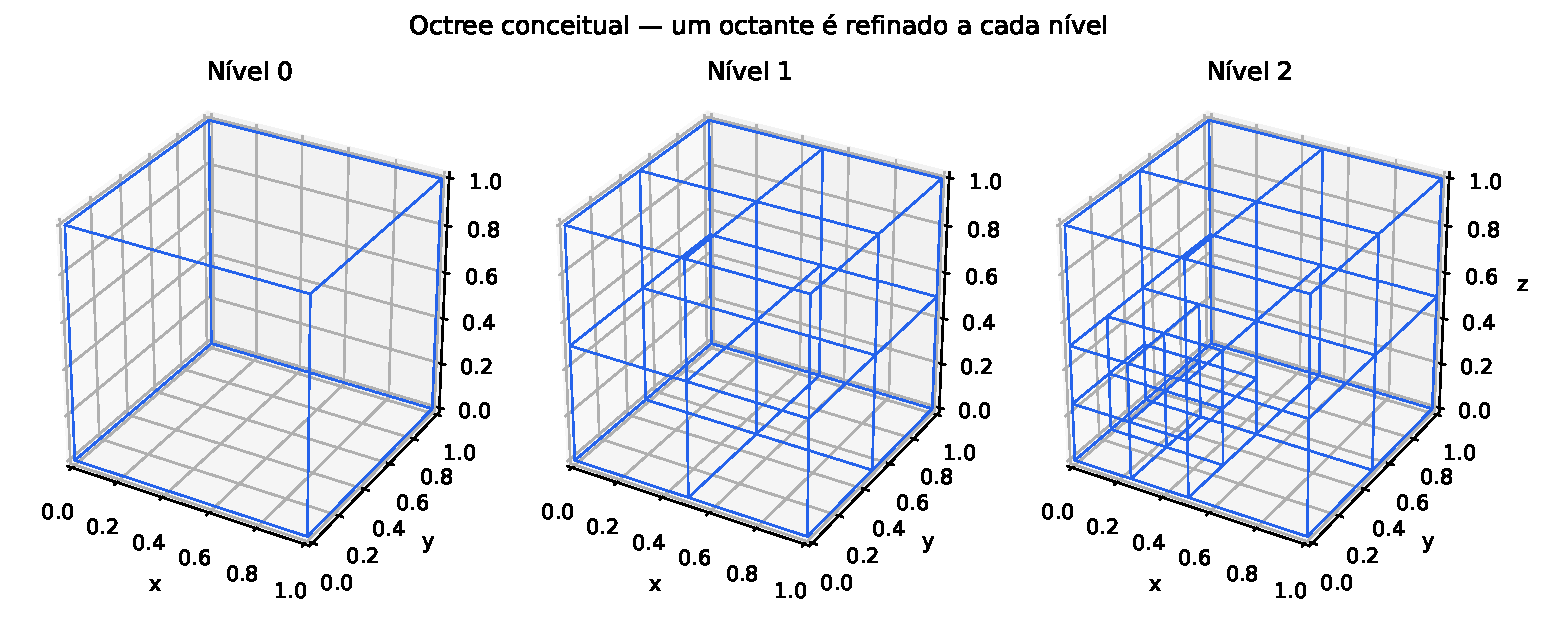
\includegraphics[width=0.98\linewidth]{figuras/metodologia_octree.pdf}
\caption{Arquitetura tabular e subdivisão hierárquica conceitual. A implementação utiliza grade de resolução fixa.}
\end{figure}

\chapter{Trabalhos Relacionados}\label{cap:relacionados}



A revisão reuniu trabalhos sobre navegação de drones, profundidade monocular, fluxo óptico, integração visual-inercial, aprendizado aplicado à percepção e explicabilidade. A busca priorizou artigos recentes e referências clássicas necessárias para explicar os métodos utilizados. A seleção não é apresentada como uma revisão sistemática. Seu objetivo é posicionar a pergunta investigada e comparar escolhas próximas às deste trabalho.

\section{Navegação e desvio com visão}

Loquercio et al. aproximam percepção e planejamento para realizar voos rápidos em ambientes naturais e artificiais \cite{Loquercio2021}. Richter et al. tratam a incerteza sobre regiões ainda não observadas durante a navegação \cite{BayesianLearning2015}. Bhattacharya et al. usam visão monocular baseada em eventos para desvio reativo \cite{Bhattacharya2024}.

Esses trabalhos avaliam o comportamento de sistemas de navegação ou políticas de voo. O presente estudo usa a navegação reativa como fonte de dados, mas concentra a avaliação na relação entre sinais sincronizados e mudanças de proximidade.

\section{Profundidade monocular}

Revisões recentes organizam métodos de profundidade monocular e apontam avanços em redes profundas \cite{Vyas2022,Arampatzakis2024,Dhanushkodi2025}. Dong et al. discutem o equilíbrio entre precisão, robustez e velocidade em aplicações em tempo real \cite{RealTimeMonocular2022}. Liu et al. tratam a incerteza da estimativa \cite{Liu2023}. O Depth Anything V2 amplia essa linha com modelos de diferentes tamanhos e ajuste para profundidade métrica \cite{DepthAnythingV2}.

Diferentemente desses trabalhos, a primeira etapa desta pesquisa não tenta produzir diretamente um mapa completo de profundidade a partir da imagem. Ela usa a profundidade do simulador como referência para avaliar se atributos mais simples acompanham sua variação temporal. A etapa espacial acrescenta um teste de utilidade: uma variante métrica do Depth Anything V2 é ajustada com dados do cenário, avaliada em execuções reservadas e transformada em mapa de ocupação antes de qualquer autorização para voo. Assim, um bom erro por pixel não basta. A estimativa também precisa evitar falsos espaços livres e produzir caminhos executáveis sem colisão no mapa de referência.

\section{Avaliação da profundidade pelo uso posterior}

O MoNA Bench compara estimadores de profundidade em tarefas de desvio e acompanhamento de alvo \cite{Pan2024MoNA}. O MonoNav combina profundidade monocular, reconstrução e planejamento em um pequeno UAV \cite{Simon2024MonoNav}. Ambos mostram aplicações da profundidade na navegação e servem de referência para a avaliação espacial deste estudo.

Wu et al. analisam a sensibilidade das métricas a perturbações geométricas e identificam limitações na avaliação da forma reconstruída \cite{Wu2025DepthEvaluation}. Em um contexto diferente, Gurram e López encontram correspondência entre métricas de profundidade e o desempenho posterior de detecção 3D \cite{Gurram2023DepthMetrics}. Os resultados mostram que a utilidade das métricas depende da tarefa. Uma correlação de desempenho em detecção não estabelece um critério suficiente para autorizar navegação.

No cenário simulado \texttt{baylands}, utilizado nos experimentos, este trabalho examina as configurações que atenderam aos limites de erro de profundidade, mas reprovaram na avaliação de ocupação e planejamento. A comparação com os artigos considera as escolhas de método, pois seus protocolos não permitem comparar diretamente os números. As versões v12--v19 são ajustes de uma mesma família de modelos.

\section{Fluxo óptico e informação inercial}

Xiao et al. combinam divergência de fluxo e dados inerciais para prevenir colisões \cite{Xiao2021}. Hu et al. aprendem o desvio a partir do movimento dos pixels \cite{PixelMotion2025}, enquanto Deng et al. combinam fluxo translacional e uma máscara de incerteza \cite{Deng2026}. Ng et al. analisam a incerteza das correspondências do fluxo \cite{Estimation2109}.

Esses estudos mostram que o fluxo carrega informação de movimento e proximidade, mas também reforçam a necessidade de considerar o movimento próprio. A diferença deste trabalho está no protocolo de dados: fluxo, IMU, deslocamento, comandos e profundidade de referência são reunidos no mesmo intervalo e avaliados por grupos.

Os resultados numéricos não são colocados lado a lado porque cada estudo usa sensores, cenas, saídas e divisões experimentais diferentes. A Tabela~\ref{tab:comparacao-relacionados} compara apenas dimensões de método que podem ser verificadas sem supor equivalência entre métricas.

\begin{table}[htb]
\centering
\caption{Comparação qualitativa com linhas de trabalhos relacionados.}
\label{tab:comparacao-relacionados}
\resizebox{\textwidth}{!}{%
\begin{tabular}{p{3.0cm}p{2.5cm}p{3.2cm}p{2.5cm}p{2.6cm}}
\hline
\textbf{Linha} & \textbf{Cenário} & \textbf{Entrada e saída} & \textbf{Validação espacial} & \textbf{Busca} \\
\hline
Loquercio et al. \cite{Loquercio2021} & natural e artificial & imagem para política de voo & desempenho em voo & integrado à política \\
Profundidade monocular \cite{DepthAnythingV2} & bases visuais diversas & RGB para profundidade & métricas por pixel & não é o foco \\
Fluxo visual-inercial \cite{Xiao2021} & navegação de UAV & fluxo e inércia para risco & prevenção de colisão & reação local \\
MoNA Bench \cite{Pan2024MoNA} & navegação de UAV & RGB para profundidade & desvio e acompanhamento & integrado às tarefas \\
MonoNav \cite{Simon2024MonoNav} & voo em ambiente interno & RGB e poses para mapa & navegação em hardware & primitivas de movimento \\
Este trabalho & Gazebo, \texttt{baylands} & sinais para proximidade; RGB para profundidade & ocupação, falso livre e colisão discreta & A* como portão posterior \\
\hline
\end{tabular}}
\legend{Fonte: elaborado pelo autor a partir dos trabalhos citados.}
\end{table}

\section{Posicionamento do trabalho}

Os trabalhos apresentados já avaliam profundidade na navegação e discutem as limitações das métricas geométricas. Este estudo acrescenta um caso em que os registros permitem acompanhar os resultados e os motivos para bloquear a integração monocular ao voo. A contribuição está na análise experimental desse caso, e não na criação da sequência câmera, mapa e planejamento.

O estudo defende que a avaliação anterior ao voo deve considerar o mapa, a disponibilidade de caminhos e a verificação de colisões, além do erro por pixel. A análise tabular investiga os sinais usados para prever mudanças de proximidade. A análise espacial verifica o uso da profundidade pelo planejador. Os dois experimentos respondem a perguntas diferentes; a ablação das entradas tabulares não foi usada para modificar o estimador de profundidade.

O protocolo pode ajudar pesquisadores que integram estimadores de profundidade a mapas e planejadores. Os resultados indicam quais sinais merecem mais investigação e quais configurações ainda não atendem aos critérios de uso definidos no experimento. Essas conclusões ficam restritas aos dados e às condições avaliadas.


A odometria visual estima o movimento da câmera a partir de imagens sucessivas. Neste estudo, a pose é fornecida pelo registro do PX4, sem implementação de odometria visual própria.





A retropropagação fundamenta o treinamento de redes multicamadas \cite{Rumelhart1986}. Random Forest e Extra Trees são métodos de conjuntos de árvores com mecanismos distintos de aleatorização \cite{Breiman2001,Geurts2006}. Grad-CAM explica regiões de imagens, sem equivaler ao gradiente local de atributos tabulares \cite{Selvaraju2017}. Comparações pareadas e tamanhos de efeito devem explicitar sua unidade de repetição \cite{Lakens2013}. A arquitetura de comunicação ROS~2 é descrita por Macenski et al. \cite{Macenski2022}.
